\section{Competitions}

\subsection{Common}

\subsubsection{Answer a question.} 
Once the contest has started, the user can read the first question. Beneath each question, the user may write his answer in the corresponding input box or he can just select the right answer in case of multiple choice. After answering the question, the user will automatically be brought to the next question. But when the user has filled in his answer in the input box, his answer will be checked against a certain pattern. This way there is some sort of check whether the user fills in something useful. If the answer does not match with the pattern, a warning text will appear above the input box, stating that the user has to change his answer in something useful and the user will not be brought to the next question until his answer checks off. The question that has been answered will be marked as answered in the question list.

\subsubsection{Navigate between questions.} 
As stated before, when the users answers the current question, he will be brought to the next question. However, during the contest the user will always see the list with all the questions in the question set of the contest. Each question will be presented with his title. Clicking on one of these titles will bring the user to the corresponding question. The user will also be able to go to the next or previous question by clicking on an arrow. 

\subsubsection{Change answer.} 
The user can change his answer to a specific question. First he navigates to the question as explained before. Then he can see his current answer and, if still preferred, change his answer. 

\subsubsection{Remove answer.} 
If the user wants to remove his answer to a specific question, he can press a button that will be positioned next to the answer possibilities. Pressing this button will remove his answer to the question. The question will no longer be marked as answered in the questions list.

\subsubsection{See time left.} 
During the contest, the time remaining will be shown. This makes it easy for the users to see how much time they've got left. 

\subsubsection{Finish a contest.} 
When the user answers the last question, he will not be brought to the next question. Instead, there will be a finish button that the user can click when he wants to finish. After pressing this button, a warning window will appear stating how much time the user got left and asking whether he wants to review his answers or not. He can then press the cancel button to review his answers or press the ok button to finish the contest. Beneath the list of questions, there will also be the same finish button. This makes it easy for the user to finish the contest when he is currently not answering the last question. 

\subsubsection{See questions that already have been answered.} 
In the list with questions, each question will be marked with some sort of sign to indicate whether the user has already answered this question or not. 

\subsubsection{See how many points that can be gained or lost.}
Just like the time remaining, the user can always see for each question how many points he can win or lose. This makes it a bit more easy for the user to know the importance of each question. 

\subsubsection{Example}
An example of how the contest page could look like \ref{Contest}.
		\begin{figure}[h]
		  \centering
			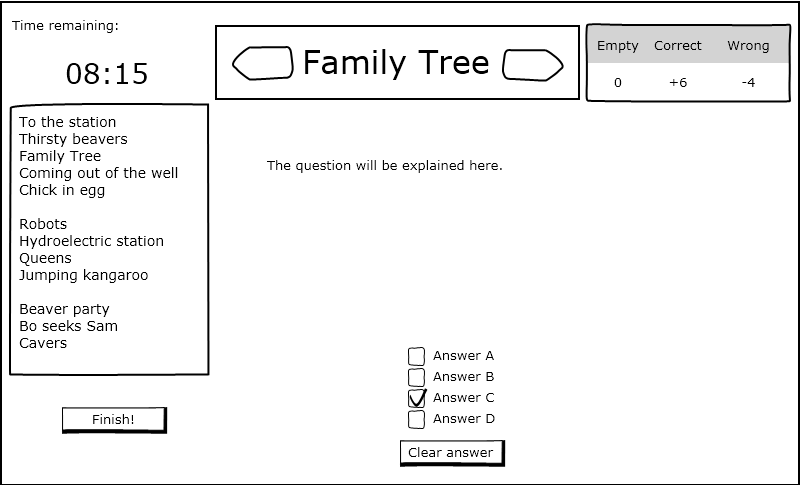
\includegraphics[width=1\textwidth]{contests.png}
		  \caption{Contest}
		  \label{Contest}
		\end{figure}

\subsection{Unrestricted contest}

\subsubsection{See results and feedback}
Immediately after finishing the contest, the user will be shown an overview that tells him how well he did on the contest. He can see the list with questions and next to each question he can see his result. Beneath the list with questions, the user can see his total score for the contest. Each question in the list will be clickable. Clicking on one of these will bring the user to the feedback page. On this page the user will be able to reread the question, to see the correct answer together with some sort of explanation and to get more information about this question.  

		\begin{figure}[h]
		  \centering
			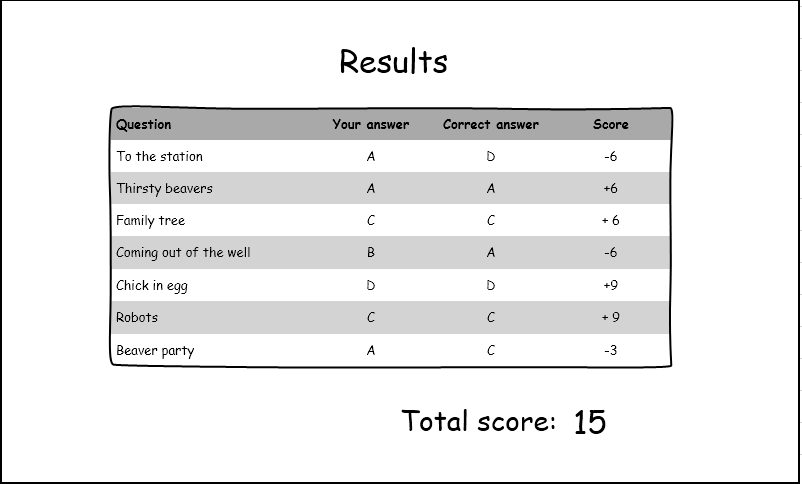
\includegraphics[width=1\textwidth]{results.png}
		  \caption{Contest}
		  \label{Contest}
		\end{figure}

\subsubsection{When the internet fails}
When the internet fails during an unrestricted contest, the user can retake the same contest when his internet connection is back running. He can rechoose the contest like he did previously and start over. 

\subsection{Restricted contest}

\subsubsection{See results and feedback}
After taking a restricted contest, the student can't see his results immediately. The result can be made available by the teacher who started the restricted contest. 

\subsubsection{When the internet fails}
When the internet fails during a restricted contest, the student can't do much about it. However the teacher is able to let the student continue the contest. The teacher can obtain a cookie with information about the answers the student had already given by pressing a button on the student's pc. He can then submit this cookie and let the student continue where he left off. The teacher can also give the student an optional amount of grace time. How this is done is explained in the teacher part. In case the internet fails during a long period, this cookie can be used by the teacher to obtain some sort of partial marking. 

\subsection{Official contest}

\subsubsection{See results and feedback}
After finishing an official contest, the student will not be able to see his results nor can he see the feedback pages. The student can see his results and the corresponding feedback pages after the official contest has been closed by the organizers. 

\subsubsection{When the internet fails}
Simular to restricted contests. 


